%%%%%%%%%%%%%%%%%%%%%%%%%%%%%%%%%%%%%%%%%%%%%%%%%%%%%%%%%%%%%%%%%%%%%%%%
%    INSTITUTE OF PHYSICS PUBLISHING                                   %
%                                                                      %
%   `Preparing an article for publication in an Institute of Physics   %
%    Publishing journal using LaTeX'                                   %
%                                                                      %
%    LaTeX source code `ioplau2e.tex' used to generate `author         %
%    guidelines', the documentation explaining and demonstrating use   %
%    of the Institute of Physics Publishing LaTeX preprint files       %
%    `iopart.cls, iopart12.clo and iopart10.clo'.                      %
%                                                                      %
%    `ioplau2e.tex' itself uses LaTeX with `iopart.cls'                %
%                                                                      %
%%%%%%%%%%%%%%%%%%%%%%%%%%%%%%%%%%
%
%
% First we have a character check
%
% ! exclamation mark    " double quote  
% # hash                ` opening quote (grave)
% & ampersand           ' closing quote (acute)
% $ dollar              % percent       
% ( open parenthesis    ) close paren.  
% - hyphen              = equals sign
% | vertical bar        ~ tilde         
% @ at sign             _ underscore
% { open curly brace    } close curly   
% [ open square         ] close square bracket
% + plus sign           ; semi-colon    
% * asterisk            : colon
% < open angle bracket  > close angle   
% , comma               . full stop
% ? question mark       / forward slash 
% \ backslash           ^ circumflex
%
% ABCDEFGHIJKLMNOPQRSTUVWXYZ 
% abcdefghijklmnopqrstuvwxyz 
% 1234567890
%
%%%%%%%%%%%%%%%%%%%%%%%%%%%%%%%%%%%%%%%%%%%%%%%%%%%%%%%%%%%%%%%%%%%
%
\documentclass{iopart}
  \expandafter\let\csname equation*\endcsname\relax
  \expandafter\let\csname endequation*\endcsname\relax
%\newcommand{\gguide}{{\it Preparing graphics for IOP journals}}
%Uncomment next line if AMS fonts required
%\usepackage{iopams}
\usepackage{graphicx}
\usepackage{amsmath}
\usepackage{ulem}
\usepackage{amssymb}
\usepackage{caption}
\captionsetup{compatibility=false}
\usepackage{subcaption}

\DeclareMathOperator{\Var}{Var}
\DeclareMathOperator{\sinc}{sinc}
\newcommand{\abs}[1]{\ensuremath{\left|#1\right|}}
\newcommand{\expect}[1]{\ensuremath{\left<#1\right>}}
\newcommand{\ket}[1]{\ensuremath{\left|#1\right>}}

\begin{document}

\title{Large squeezing in multicomponent trapped Bose-Einstein condensates}

\author{Mattias T Johnsson$^1$, Graham R Dennis$^2$ and Joseph J Hope$^1$}

\address{$^1$Department of Quantum Science, Research School of Physics and Engineering, The Australian National University, Canberra ACT 0200, Australia}
\address{$^2$Plasma Research Laboratory, Research School of Physics and Engineering, The Australian National University, Canberra ACT 0200, Australia}
\ead{mattias.johnsson@anu.edu.au}

\begin{abstract}
We examine the feasibility of creating and measuring large relative number squeezing in multicomponent trapped Bose-Einstein condensates.  In the absence of multimode effects, this squeezing can be arbitrarily large, but a range of processes limit the measurable squeezing in realistic trap configurations.  We examine these processes, and suggest methods to mitigate them. We conclude that high levels of squeezing with large numbers of atoms is feasible, but can realistically only be achieved in traps with even density profiles in at least two dimensions. We also introduce a method of maximising the measurable squeezing by using a pi-pulse during the process to improve spatial mode-matching.
\end{abstract}

%Uncomment for PACS numbers title message
%\pacs{00.00, 20.00, 42.10}
% Keywords required only for MST, PB, PMB, PM, JOA, JOB? 
%\vspace{2pc}
%\noindent{\it Keywords}: Article preparation, IOP journals
% Uncomment for Submitted to journal title message
%\submitto{\JPA}
% Comment out if separate title page not required
\maketitle

\section{Introduction}
\label{sectionIntroduction}
\begin{itemize}
  \item General non-classical state generation with atoms
  \item Talk about number squeezing with atoms
  \item Link to interferometry
  \item Motivate why large number squeezing
  \item Point out no one has done it before, only low number squeeze
  \item Lay out what sections we have and what we've done
\end{itemize}

\section{Model and two mode solutions}
\label{secTwoModeAnalytic}
Our goal is to describe the number squeezing possibilities of a BEC comprising two relevant internal states denoted by $|a\rangle$ and $|b\rangle$.  The Hamiltonian for a pair of coupled atomic internal modes is the spatial integral of the Hamiltonian density, which is given by
\begin{equation}
\hat{\mathcal{H}} = \sum_{j} \hat{\psi}_j^{\dagger}\left(-\frac{\hbar^2}{2 m}\nabla^2+V_j\right)\hat{\psi}_j 
          + \sum_{i j}\frac{U_{i j}}{2} \hat{\psi}_i^{\dagger} \hat{\psi}_j^{\dagger} \hat{\psi}_j \hat{\psi}_i
          + \kappa \hat{\psi}_a^{\dagger} \hat{\psi}_b + \kappa^* \hat{\psi}_b^{\dagger}  \hat{\psi}_a
\label{eqFieldHamiltonian}
\end{equation}
where $\hat{\psi}_j(\mathbf{x})$ is the annihilation field operator for a particle at position $\mathbf{x}$ and in internal state $|j\rangle$, $m$ is the mass of the atoms, $V_j(\mathbf{x})$ is the trapping potential for atoms in internal state $|j\rangle$, $U_{ij}$ describe the various inter- and intra-state nonlinearities, and $\kappa$ describes the coupling between the two states.  

We begin by considering a simplified version of the problem, assuming that only one of these spatial modes is relevant for each of the condensate's components.  This is done by writing the multimode atomic field operators in terms of a set of basis functions $\hat{\psi}_a({\mathbf{r}},t) = \sum_n u_{n}({\mathbf{r}}) \hat{a}_{n}(t)$ and $\hat{\psi}_b({\mathbf{r}},t) = \sum_n u_{n}({\mathbf{r}}) \hat{b}_{n}(t)$, where $\hat{a}_{n}$ and $\hat{b}_{n}$ annihilate a particle with normalised spatial mode $u_n$ and internal state $|a\rangle$ or $|b\rangle$ respectively. With this expansion, the first nonlinear term in the multimode Hamiltonian becomes
\begin{equation}
\hat{H} = \frac{U_{aa}}{2} \int dV \sum_{nmpq} u_n^* u_m^* u_p u_q \, \hat{a}^{\dagger}_{n} \hat{a}^{\dagger}_{m} \hat{a}_{p} \hat{a}_{q} 
\end{equation}
When the system remains predominantly in one mode, we can approximate this sum as the single term $\hat{H} = \chi_{aa} \hat{a}^{\dagger} \hat{a}^{\dagger} \hat{a} \hat{a}/2$ where
\begin{equation}
\chi_{aa} = U_{aa} \int |u_i|^4 \, dV.
\label{eqChiUequivalence}
\end{equation}
We proceed similarly for the other terms.  In the parameter regimes we are interested in, the detuning between the two spatial modes will be irrelevant, so setting our zero of energy appropriately, we are left with only a standard Kerr-type nonlinearity arising from atom-atom interactions, as well as a linear coupling between the two modes.  The Hamiltonian governing this reduced system is given by
\begin{equation}
\hat{H} = \frac{\chi_{aa}}{2} \hat{a}^{\dagger} \hat{a}^{\dagger} \hat{a} \hat{a}
          + \chi_{ab} \hat{a}^{\dagger} \hat{a} \hat{b}^{\dagger} \hat{b}
          + \frac{\chi_{bb}}{2} \hat{b}^{\dagger} \hat{b}^{\dagger} \hat{b} \hat{b}
          + \Omega (\hat{a}^{\dagger} \hat{b} + \hat{b}^{\dagger}  \hat{a} )
\label{eqTwoModeHamiltonian}
\end{equation}
where the $\chi_{ij}$ describe the various inter- and intra-mode nonlinearities, and $\Omega$ couples the two modes and allows for population transfer between them.

The system is prepared with all the population in $|a\rangle$, and vacuum in $|b\rangle$. We choose state $|a\rangle$ to be occupied as a coherent state with average number $\langle \hat{a}^{\dagger} \hat{a} \rangle = N$, where $N$ is the total particle number in our system.  As our simulation and experiment are insensitive to the initial phase of the coherent state, this is equivalent to a mixture of coherent states of uncertain phase, which is also equivalent to mixture of Poissonian-distributed number states.  This state is consistent with BEC coherence experiments \cite{Hadzibabic2004}.  

At time $t=0$ the coupling $\Omega$ is switched on and applied until time $t=t_1$, at which point it is turned off, resulting in a portion of the population being transferred into mode $|b\rangle$. As the initial state was a coherent state in both modes, after the population transfer both $|a\rangle$ and $|b\rangle$ are described by coherent states, with mean number $\langle \hat{a}^{\dagger} \hat{a} \rangle = n_a$ and $\langle \hat{b}^{\dagger} \hat{b} \rangle = n_b$ respectively.

The coupling $\Omega$ is then switched off until time $t_2$. During this period the atoms interact solely through the nonlinear terms, with no population being transferred. Due to the form of the Hamiltonian, the number variance remains unchanged, but the quadrature variances in the two modes change over time, which can lead to quadrature squeezing \cite{johnssonET2007}.

After this hold time $\tau_{\mathrm{hold}} = t_2 - t_1 $, the coupling $\Omega$ is switched back on until time $t_3$, with a phase shift $\phi$ compared to its first application. During this last stage, the two modes exchange population and the quadrature variance is converted into number variance, in the same way homodyne measurements are used in quantum optics to convert quadrature squeezing into number squeezing, which can be directly measured. In this interpretation, $\phi$ is the relative phase of the strong local oscillator, which allows specific phase angles of quadrature squeezing to be examined.  This experiment can also be interpreted as a Ramsey interferometer with a final beam splitter phase of $\phi$.

The entire sequence of pulses and the resulting populations are shown schematically in Figure~\ref{figPulseScheme}.

\begin{figure}
    \centering
    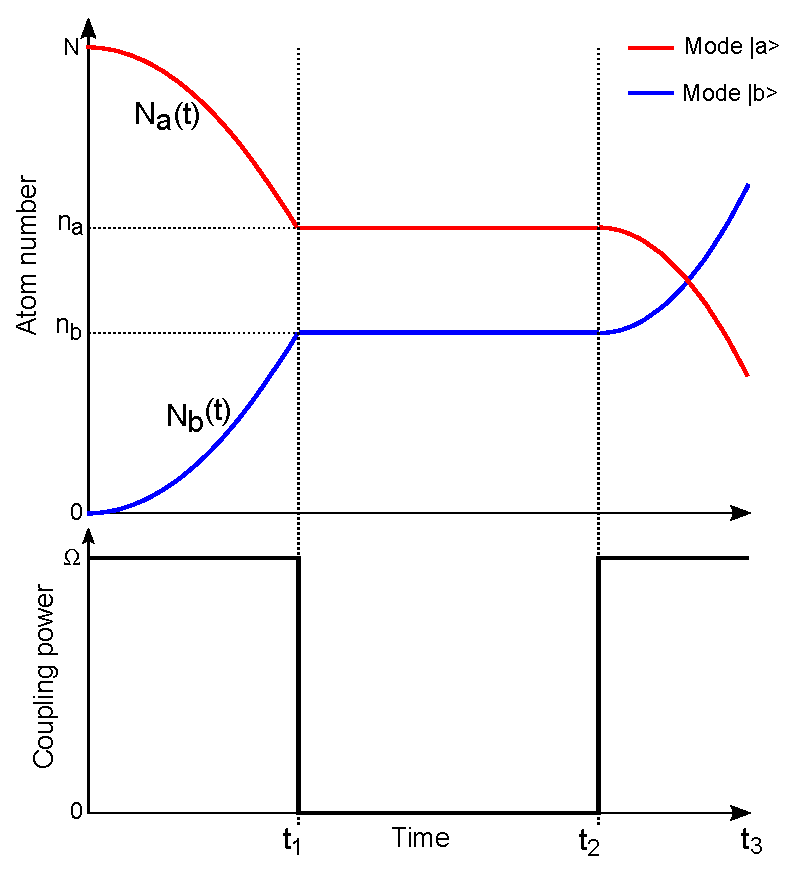
\includegraphics[width=8cm]{figures/pulse_scheme.eps}
    \caption{Schematic of the pulse sequence and atomic populations as a function of time.  Typically the coupling sequences at the beginning and end of the sequence are much shorter than the hold time, $\tau_{\mathrm{hold}} = t_2 - t_1 $, which is where the majority of the squeezing occurs.}
    \label{figPulseScheme}
\end{figure}

This system can be solved analytically, and expressions for quadrature, absolute and relative number squeezing can be derived. We present the solutions here; the full derivation can be found in \ref{appendixTwoModeDerivation}.
If we define
\begin{eqnarray}
s &=& \sin(\Omega (t_3 - t_2)) \label{eqsDef} \\
c &=& \cos(\Omega (t_3 - t_2)) \\
\lambda_{ij} &=& \chi_{ij} \tau_{\mathrm{hold}} / \hbar \\
A &=& \sqrt{n_a} \exp [n_a (e^{-i(\lambda_{aa}-\lambda_{ab})} - 1 )] \\
A_2 &=& n_a \exp [n_a (e^{-2i(\lambda_{aa}-\lambda_{ab})} - 1 )] \\
B &=& -i e^{i \phi}\sqrt{n_b} \exp [n_b (e^{-i(\lambda_{bb}-\lambda_{ab})} - 1 )] \\
B_2 &=& -n_b e^{2i\phi} \exp [n_b (e^{-2i(\lambda_{bb}-\lambda_{ab})} - 1 )] \\
D &=& AB^* - A^*B \label{eqDDef}
\end{eqnarray}
then the expectation values for number, number variance, and number difference variance after appling the final coupling field are given by
\begin{eqnarray}
N_a(t_3) &=& n_a c^2 + n_b s^2 + i c s D \\
%
N_b(t_3) &=& n_a s^2 + n_b c^2 - i c s D \\
%
{\mathrm{Var}} [ N_a](t_3) &=& n_a c^2 + n_b s^2 + 2 n_a n_b c^2 s^2 \\
       && + c^2 s^2 (D^2 - e^{i(\lambda_{aa} - \lambda_{bb})} B_2 A_2^* - e^{-i(\lambda_{aa} - \lambda_{bb})} B_2^* A_2) \nonumber \\
       && + i c s D (1-2 n_a c^2 -2 n_b s^2)  \nonumber\\
       && + 2 i c^3 s n_a (e^{-i(\lambda_{aa} - \lambda_{ab})} A B^* - e^{i(\lambda_{aa} - \lambda_{ab})} A^* B ) \nonumber \\
       && + 2 i c s^3 n_b (e^{i(\lambda_{bb} - \lambda_{ab})} A B^* - e^{-i(\lambda_{bb} - \lambda_{ab})} A^* B ) \nonumber\\
%
{\mathrm{Var}} [ N_b](t_3) &=&  n_a s^2 + n_b c^2 + 2 n_a n_b c^2 s^2 \nonumber \\
       && + c^2 s^2 (D^2 - e^{i(\lambda_{aa} - \lambda_{bb})} B_2 A_2^* - e^{-i(\lambda_{aa} - \lambda_{bb})} B_2^* A_2 ) \nonumber \\
       && + i c s D (-1+2 n_a s^2 + 2 n_b c^2)  \nonumber \\
       && + 2 i c^3 s n_b (e^{-i(\lambda_{bb} - \lambda_{ab})} A^* B - e^{i(\lambda_{bb} - \lambda_{ab})} A B^* ) \nonumber \\
       && + 2 i c s^3 n_a (e^{i(\lambda_{aa} - \lambda_{ab})} A^* B - e^{-i(\lambda_{aa} - \lambda_{ab})} A B^* ) \\
%
{\mathrm{Var}} [ N_a - N_b](t_3) &=& n_a + n_b + 4 i c s D (n_a - n_b)(s^2 - c^2) \nonumber \\
       && + 4 c^2 s^2 (2 n_a n_b +D^2 - e^{i(\lambda_{aa} - \lambda_{bb})} A_2^* B_2 - e^{-i(\lambda_{aa} - \lambda_{bb})} A_2 B_2^* ) \nonumber \\
       && + 4 i c s (c^2 - s^2) (n_a e^{-i(\lambda_{aa} - \lambda_{ab})} A B^* - n_a e^{i(\lambda_{aa} - \lambda_{ab})} A^* B 
                     + n_b e^{-i(\lambda_{bb} - \lambda_{ab})} A^* B - n_b e^{i(\lambda_{bb} - \lambda_{ab})} A B^*) \label{eqNumDiffVariance}
\end{eqnarray}
In the case where all the nonlinearities are equal, such that $\chi_{aa} = \chi_{ab} = \chi_{bb}$, the number variances all reduce to those of a coherent state, e.g. ${\mathrm{Var}}[N_a]=N_a$, and no number squeezing is possible. It should also be noted that, although there are three independent nonlinearities $\chi_{ij}$ in the Hamiltonian (\ref{eqTwoModeHamiltonian}), the expressions for the number variances only depend on differences. This means that number squeezing is parameterised by only two independent quantities, for example $\chi_{aa}-\chi_{ab}$ and $\chi_{aa}-\chi_{bb}$.  

%Can Uaa + Ubb - 2Uab be zero and still get squeezing? Yep, Uaa=0.03, Ubb=0.01, Uab=0.02 gives squeezing for all quantities of interest

While the analytic expressions for the number variances are not particularly edifying, it is easy to evaluate and plot them for any given set of parameters. As an example, in Figure \ref{figTwoModeAnalyticExamples} we plot the solution for the normalized number variance in mode $|a\rangle$ for a particular set of nonlinearities, choosing a number of different values of $\phi$. The plots illustrate the basic features of the problem: During the final coupling period, the normalised number variance undergoes cyclic variation with a period $\tau=\pi / \Omega$, and has a series of minima. It is necessary to choose both the correct phase $\phi$ as well as the correct length of time for the coupling to be applied in order to obtain optimum squeezing.

This two-mode analytic model allows arbitrarily good number squeezing, provided there are no limits to the number of particles in the system or to the hold time. Unfortunately, in any realistic system, there are more than two modes present, and multimode effects conspire to limit the level of squeezing that can be achieved. It is to this that we now turn.

\begin{figure}
    \centering
    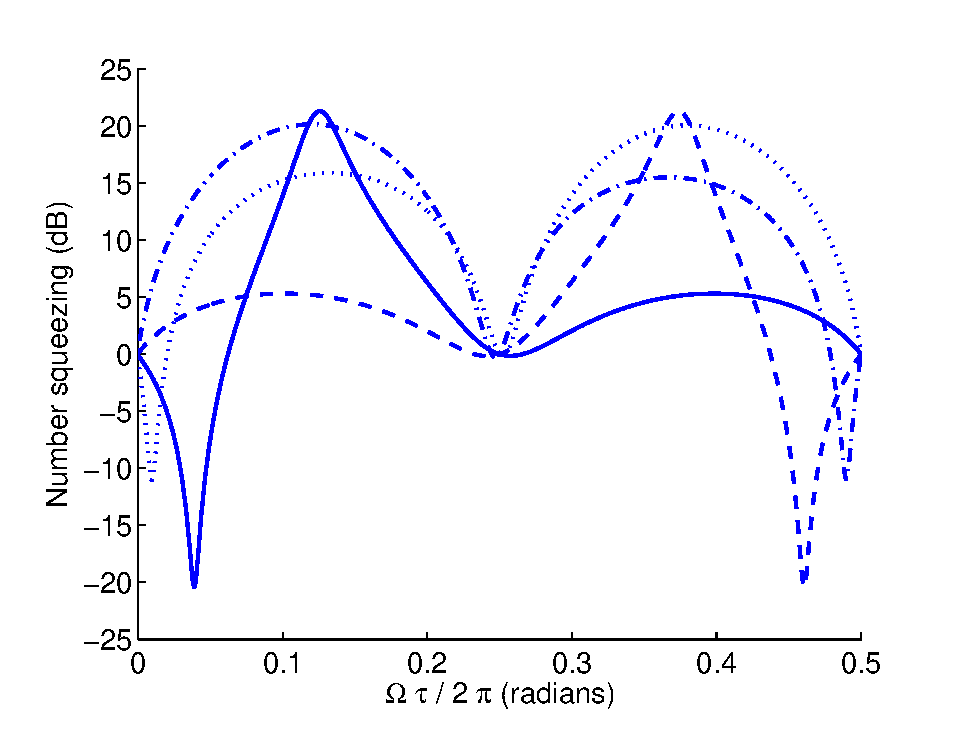
\includegraphics[width=10cm]{figures/analytic_two_mode_examples.eps}
    \caption{Normalized number variance Var$[N_a]/N_a$ in mode $|a \rangle$ as a function of final recombination time plotted on a logarithmic scale, using four different mixing angles $\phi$. Parameters: $n_a = n_b =5 \times 10^5$, $\chi_{aa}=0.04 \hbar, \chi_{ab}=0, \chi_{bb}=0.01\hbar, \tau_{\mathrm{hold}}=4\times 10^{-4}$s. Solid line, $\phi=0.10$; dash-dotted line, $\phi=1.42$; dashed line, $\phi=3.24$; dotted line, $\phi=4.71$. These particular parameters yield 21dB of number squeezing for the $\phi=0.1$ and $\phi=1.42$ cases.} 
    \label{figTwoModeAnalyticExamples}
\end{figure}

\begin{itemize}
  \item Maybe point out it agrees with Oberthaler, or save that for discussion on MM effects?
  \item Point out that number *difference* squeezing can often be considerably higher than absolute number squeezing in a single state
\end{itemize}


\section{Multimode number squeezing analysis} \label{sec:MMdescription}

The zero-dimensional, two-mode model described in the previous section shows that arbitrarily high squeezing can be achieved using the intrinsic nonlinearities in a BEC, but it ignores the existence of multiple spatial modes.  There are three problems caused by the existence of multiple modes, and these will limit the achievable squeezing.

The first problem is present even if the spatial modes are uncoupled.  The two-mode model shows that the parameters required to obtain best squeezing are dependent on the strength of the nonlinearity. In the multimode case, the effective nonlinearity of a mode is a function of the mode shape, as is shown by Eq.~(\ref{eqChiUequivalence}). The optimum hold time $\tau_{\mathrm{hold}}$ depends on the product of the effective mode nonlinearity and number number of particles in that mode, as does the recombination phase $\phi$.  Different modes in a multimode environment will typically have varying effective nonlinearity-particle number products and therefore squeeze at different rates, with each mode having a different optimum $\tau_{\mathrm{hold}}$ and optimum recombination phase $\phi$. This means that the best squeezing will be achieved by choosing values of $\tau_{\mathrm{hold}}$ and $\phi$ that, averaged across all the spacial modes present, result in an overall lowest possible total number variance.  

The second problem is due to the number-dependent dynamics of the spatial modes, which is observable even in a semiclassical simulation.  Due to the nonlinear term in the Hamiltonian, the local phase evolution of the atomic field is density dependent.  Consequently the mode shape of the atomic field changes depending on the nonlinearity-density product, which means that unless $U_{aa}|\psi_a({\mathbf{r}})|^2 = U_{bb}|\psi_b({\mathbf{r}})|^2$ for all ${\mathbf{r}}$, the mode shapes will not overlap perfectly during the final coupling pulse. This degraded mode-matching will result in lower efficiency when converting the quadrature squeezing to number squeezing. 

We might speculate that the effects of these first two problems would be lessened by trap geometries that lead to near-constant density profiles for the BEC.  This should enable higher squeezing.  We cannot make strong conclusions without also considering the effects of coupling between spatial modes, however, which leads to the third potential problem: Coupling between modes is inevitable in the presence of a nonlinearity, meaning that the modes cannot be analyzed independently. Coupling between modes will disturb mode-matching, as well as mixing fields with different phase evolution, which can rapidly destroy squeezing.  

An analytic solution to the multimode, higher-dimensional problem is intractable, so we must use a numerical solution.  We use stochastic methods based on phase space representations to simulate the dynamics of the multimode quantum fields.  These methods alleviate the problem of directly simulating elements of the Hilbert space, the size of which increases exponentially with the number of spatial modes \cite{stochasticRefs}.  Stochastic methods achieve this by finding a sufficiently well-behaved quasi-probability representation for the density matrix, which can then be simulated as the average behaviour of a number of low-dimensional samples.  These sample objects are the same size as the equivalent classical field.  In our case, the only tractable phase space representation is the functional Wigner representation, which is well behaved when the quantum field is approximately Gaussian, as it is for coherent and squeezed states.  Stochastic methods based on the functional Wigner representation have been used to model the behaviour or BECs and atom lasers \cite{johnssonET2007,dallET2009,dennisET2010}, as the Wigner representation allows the mapping of the system to a Fokker-Plank equation (unlike the $P$-representation), and does not suffer exponential path-weighting problems that would constrain it to very short simulation intervals (as would the positive-$P$ representation).

The equation of motion for the density matrix is defined by the Hamiltonian in Eq.~(\ref{eqFieldHamiltonian}).  This defines the evolution of the functional Wigner distribution of the system, which has a one-to-one correspondence with the density matrix.  The equation of motion for the functional Wigner distribution contains derivatives of third order which we assume to be negligible.  This uncontrolled approximation is called the Truncated Wigner Approximation (TWA), and while it has been used widely on ultracold gases \cite{atomlaserWigner,orOtherUCGWigner}, care must be taken that the simulation remains valid. For our simulations we checked the results of our simulations against both the analytic two-mode solution, as well as checking for typical indications of TWA breakdown such a the appearance of negative densities in lightly populated modes. In all the regimes we investigated the TWA remained valid, apart from the most demanding simulations which took place in 3D with high nonlinearities and long hold times. The difficulty with these 3D simulations was that due to the large number of modes they included, the number of particles per mode could drop to ten or less in the densest regions where the squeezing was generated. Over very long time scales, this low mode occupation began to result in TWA breakdown. As we could characterise the regime in which breakdown began to occur, however, we were able stay away from it and to ensure our simulations remained valid.

Under the TWA, the equation of motion for the functional Wigner distribution is a Fokker-Planck equation, and can therefore be sampled by a set of stochastic equations, as described in \cite{GardinerQuantumNoise}.  These stochastic fields $\phi(\mathbf{x})$ are related to field operator expectation values by  
\begin{equation}
\langle :\hat{\psi}^\dagger(\mathbf{x_1})\cdots\hat{\psi}^\dagger(\mathbf{x_n})\hat{\psi}(\mathbf{y_1})\cdots\hat{\psi}(\mathbf{y_m}):_{\mbox{sym}}\rangle = \mathbb{E}\left[\phi^*(\mathbf{x_1})\cdots\phi^*(\mathbf{x_n})\phi(\mathbf{y_1})\cdots\phi(\mathbf{y_m})\right]
\label{eqExpectationRelations}
\end{equation}
%
where $:\star:_{\mbox{sym}}$ denotes symmetric ordering of the operators, and $\mathbb{E}$ denotes a stochastic average over the variables $\phi(\mathbf{x})$.  While we see below that the evolution of these fields is deterministic, the initial state still requires a random element, so multiple realisations are required.  When approximating these equations on a discrete grid, the magnitude of initial noise, the relationship between stochastic averages and the expectation values, and the equations of motion all become grid-dependent.  This is less concerning as it may at first appear, as the Hamiltonian in Eq.~(\ref{eqFieldHamiltonian}) assumes a contact potential between the atoms, and this is not correct below a length scale that can probe the details of the true potentials.  Furthermore, well before that regime is reached, the different elements of grid dependence cancel out to give grid-independent predictions for physical observables.

These stochastic equations take the form
\begin{eqnarray}
\frac{d \phi_a}{dt} = -\frac{i}{\hbar}\left(-\frac{\hbar^2}{2 m}\nabla^2+V_a(\mathbf{x}) + U_{a a} \left( \left|\phi_{a}\right|^2 -\frac{1}{dV}\right) + U_{a b} \left( \left|\phi_b\right|^2 -\frac{1}{2dV}\right)  \right)\phi_a   + \kappa \phi_b  \nonumber \\
\frac{d \phi_b}{dt} = -\frac{i}{\hbar}\left(-\frac{\hbar^2}{2 m}\nabla^2+V_b(\mathbf{x}) + U_{b b} \left( \left|\phi_{b}\right|^2 - \frac{1}{dV} \right) + U_{a b} \left( \left|\phi_a\right|^2 -\frac{1}{2dV} \right)   \right)\phi_b   + \kappa^* \phi_a
  \label{eqStochasticEquations}
\end{eqnarray}
where $dV$ is the volume element of the grid on which the simulation is carried out, and the terms proportional to $1/dV$ correspond to a vacuum corrections. It is a peculiarity of the Wigner representation that, up to the vacuum correction terms, Eqs.~(\ref{eqStochasticEquations}) look identical to those of the coupled semi-classical nonlinear Schr{\"{o}}dinger equation. The quantum statistical nature of the Wigner equations enters due to the fact that Eqs.~(\ref{eqStochasticEquations}) are run many times and stochastically averaged, with each run using different set of random initial conditions describing (in this case) the noise on a coherent state.


\textbf{Note the initial state we use, and the equations.}

We integrate equations (\ref{eqStochasticEquations}) numerically in one, two and three spatial dimensions using the numerical package XMDS2 \cite{dennis2013}.  For the one- and two-dimensional simulations, the dimensional reduction is achieved by estimating the mode shape in three dimensions, and using dimensionally reduced values for $U_{ij}$ that match the zero-dimensional reduction given by Eq.~(\ref{eqChiUequivalence}).  An equivalent process is to match the chemical potentials of the initial states.  

\section{Effects of trap geometries on squeezing in 1D}

A one-dimensional simulation is sufficient to examine the hypothesis that the squeezing will be higher for a BEC where the spatial mode has a more constant density profile.  We compare squeezing for fields starting in the ground states of a harmonic trap with negligible nonlinearity (a Gaussian), a harmonic trap with strong nonlinearity (Thomas-Fermi), and a constant potential (constant density). Using Eq.~(\ref{eqChiUequivalence}) we find the following equivalences
\begin{eqnarray}
\chi &=& U \sqrt{\frac{m^3 \omega_x \omega_y \omega_z}{8 \pi^3 \hbar^3}} \,\,\,\, ({\textrm{Gaussian}}) \\
%
\chi &=& \frac{4}{7} \left( \frac{15 U \omega_x \omega_y \omega_z}{16 \pi \sqrt{2}} \right)^{2/5} \left( \frac{m}{N} \right)^{3/5} \,\,\,\, ({\textrm{Thomas-Fermi}}) \\
%
\chi &=& \frac{U}{V} \,\,\,\, {\textrm{(constant density)}}
\end{eqnarray}
%
where $\omega_x$, $\omega_y$, $\omega_z$ are the angular frequencies of the harmonic trap, and $N$ is the number of particles in the mode of interest.

Choosing parameters such that the squeezing occurs fast enough that the mode shape is reasonably stable over the simulation gives the best squeezing, and allows us to make a fair comparison between the squeezing achievable by different mode shapes without being concerned that different modes will change shapes at different rates, ruining mode-matching. The results of this simulation are shown in Figure~\ref{figModalSqueezingEffects1D}, which clearly confirms the hypothesis that maximum squeezing is obtained when the mode shape is closest to constant density.

\begin{figure}
    \centering
    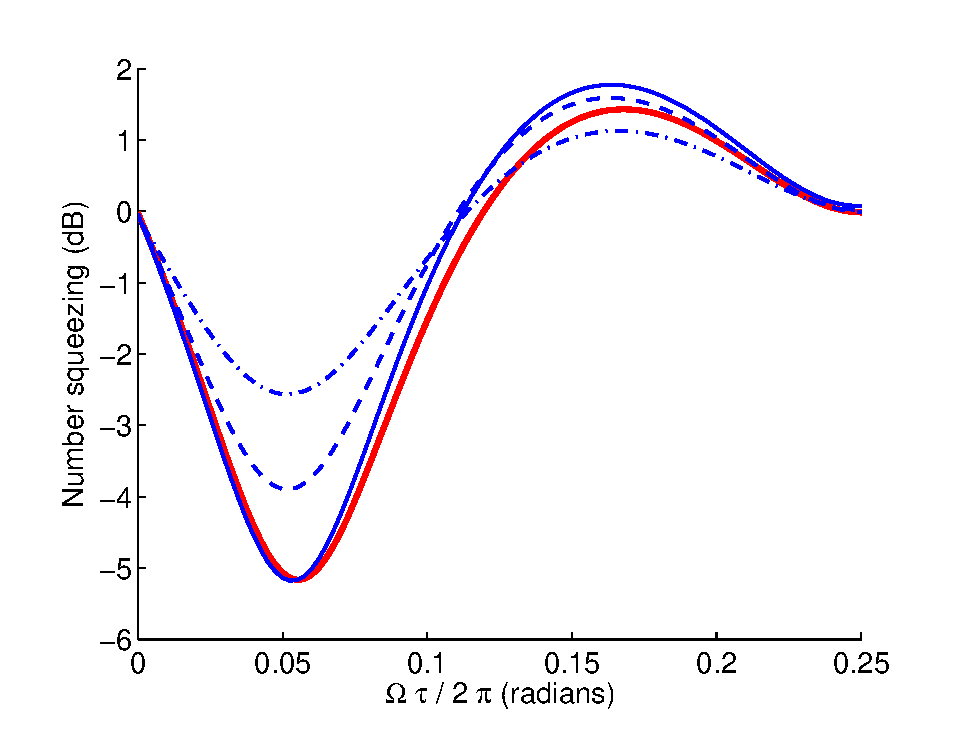
\includegraphics[width=8cm]{figures/modal_squeezing_effects_1D.eps}
    \caption{Effects of mode shape on squeezing. The plot shows the normalized number variance in mode $|a \rangle$ as a function of the time the final coupling pulse is applied. Thick red line, analytic two-mode solution; solid blue line, constant density mode; dashed line, Thomas-Fermi mode; dash-dotted line, Gaussian mode. The nonlinearities of the various 1D simulations have been adjusted for their mode shape so that they are equivalent to that of the 0D, two-mode mode nonlinearity. Parameters: $n_a = n_b =1 \times 10^5$, $\chi_{aa}=0.03 \hbar, \chi_{ab}=\chi_{bb}=0, \tau_{\mathrm{hold}}=3\times 10^{-4}$s, $\phi=4.0$. Maximum squeezing is achieved when the atomic density profile is the most uniform.}
    \label{figModalSqueezingEffects1D}
\end{figure}

One way to avoid the requirement to engineer and maintain specific atomic modes is to post-select a mode.  Rather than considering the variance in the total number of atoms in a mode, it may be possible to consider only the statistics of a spatially filtered area of the atomic cloud.  For example, suppose the atoms were in a Gaussian atomic distribution, but we consider a mode that only includes the atoms within $p$ standard deviations of the centre. For low $p$, this mode shape is considerably closer to the constant density case than a standard Gaussian. The equivalence between the single mode case and this mode is given by
\begin{equation}
\chi = U \frac{{\mathrm{Erf}} (\sqrt{2p})^3}{{\mathrm{Erf}}(p)^6} \sqrt{\frac{m^3 \omega_x \omega_y \omega_z}{8 \pi^3 \hbar^3}}
\end{equation}
A simulations comparing the best attainable squeezing for this mode compared to an unfiltered Gaussian is shown in Figure~\ref{XXX}.  We can see that the squeezing is higher.  One obvious disadvantage to post-selecting modes is that it  reduce the effective number of atoms.  This is a serious issue for most applications of squeezed sources, such as interferometry, where the signal to noise scales with the square root of the flux.

\section{Using a $\pi$-pulse to improve mode-matching}
Modal mismatch is generated by the different atomic potentials seen by the two internal states.  We propose a straightforward method of minimising this effect: using a $\pi$-pulse to swap the populations of the internal states after half of the evolution. As can be seen by Eqs~(\ref{eqa1},\ref{eqb1}, such a pulse also leaves the quantum statistics of each state unchanged. In the limit where each state stayed in a single mode (although that mode might change), and exactly half of the atoms are in each state, this method would produce identical mode shapes for both modes after the hold time. In practice this will never work perfectly as the mode shapes will change, resulting in non-identical environments for the two modes. Nonetheless, in many regimes, such a $\pi$-pulse can produce some improvement. More importantly, as this scheme accepts that the two modes will change shape, and attempts to make them change in a similar fashion, it allows the possibility of much longer hold times. That is, if we are no longer constrained to hold times short enough such that the mode shapes of the atoms in states $|a \rangle$ and $|b \rangle$ do not change significantly, much more squeezing can be extracted from the system.

These points are illustrated in Fig.~\ref{piPulseFig}, which shows the best squeezing obtainable from a specific system with and without the $\pi$-pulse, as well as the extra squeezing that can be obtained by allowing a longer hold time as well as the $\pi$-pulse.
\begin{figure}
    \centering
    \includegraphics[width=8cm]{figures/pi_pulse.eps}
    \caption{Effect of a $\pi$-pulse halfway through the hold time. Common parameters: $n_a = n_b =2 \times 10^5$, $\chi_{aa}=0.03\hbar$, $\chi_{ab}=\chi_{bb}=0$. Solid red line: Analytic two-mode solution, $\tau_{\mathrm{hold}}=3\times 10^{-4}$s, $\phi=3.0$ (10.9dB squeezing); Solid blue line: no $\pi$-pulse, $\tau_{\mathrm{hold}}=3\times 10^{-4}$s, $\phi=3.0$ (4.9dB squeezing);  Dashed blue line: with $\pi$-pulse, $\tau_{\mathrm{hold}}=3\times 10^{-4}$s, $\phi=3.05$ (5.8dB squeezing); Dash-dotted blue line: with $\pi$-pulse and the longer hold time $\tau_{\mathrm{hold}}=5\times 10^{-4}$s allowed by the application of the pulse, $\phi=3.87$ (7.2dB squeezing).}
    \label{piPulseFig}
\end{figure}

\section{Squeezing in 2D and 3D}

\begin{figure}
  \centering
  \begin{subfigure}{.5\textwidth}
    \centering
    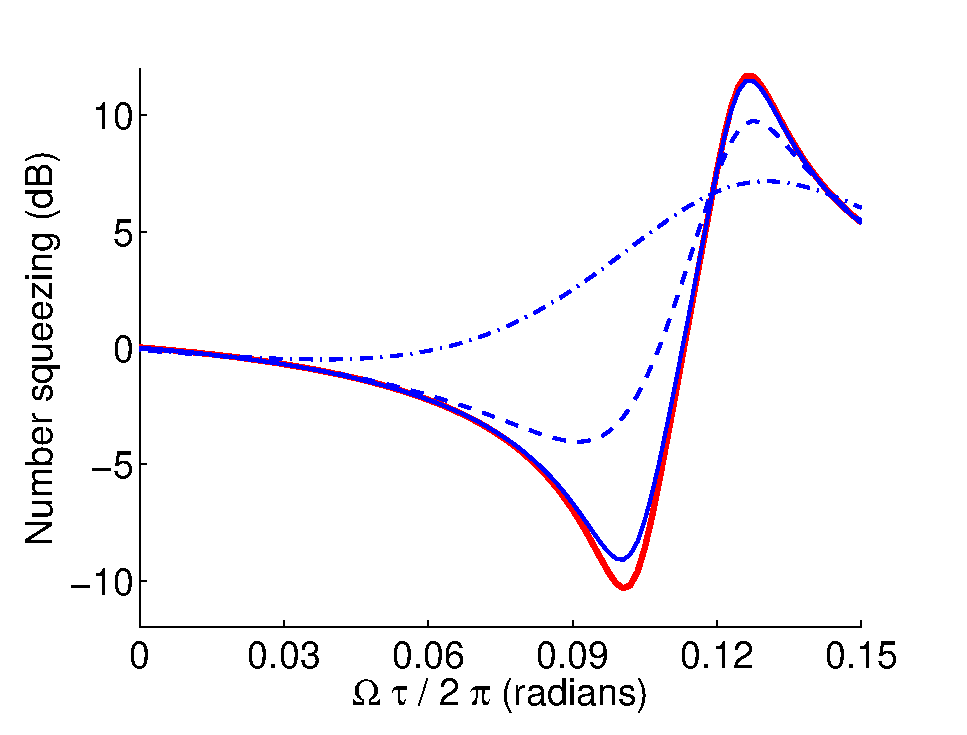
\includegraphics[width=7cm]{figures/dimensional_effects_on_squeezing_1.eps}
    \label{figDimensionalSqueezingEffects:sub1}
  \end{subfigure}%
  \begin{subfigure}{.5\textwidth}
    \centering
    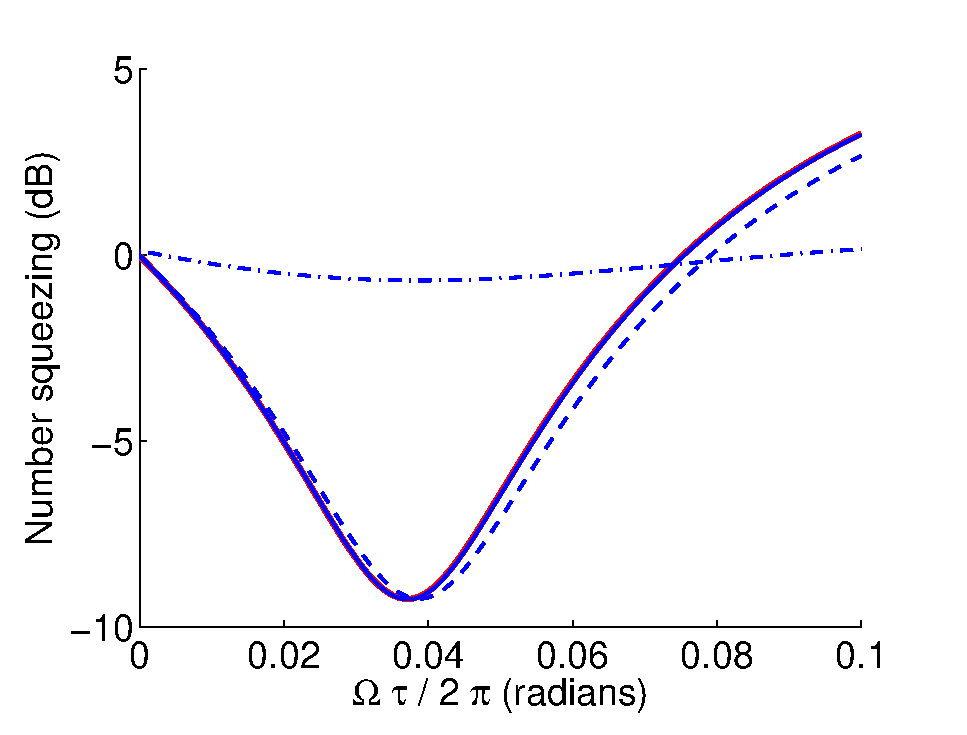
\includegraphics[width=7cm]{figures/dimensional_effects_on_squeezing_2.eps}
    \label{figDimensionalSqueezingEffects:sub2}
  \end{subfigure}
\caption{Effects of dimension on squeezing in two different nonlinear regimes. If two nonlinearities are non-zero, the deleterious effects of higher dimensions on squeezing are exacerbated. Thick red line, analytic two-mode solution; solid blue line, 1D; dashed line, 2D; dash-dotted line, 3D. (a) Parameters: $n_a = n_b =2 \times 10^5$, $\chi_{aa}=\chi_{bb}=0.03\hbar$, $\chi_{ab}=0$, $\tau_{\mathrm{hold}}=3\times 10^{-4}$s, $\phi=6.2$. (b) $n_a = n_b =2 \times 10^5$, $\chi_{aa}=0.03\hbar$, $\chi_{bb}=\chi_{ab}=0$, $\tau_{\mathrm{hold}}=3\times 10^{-4}$s, $\phi=3.1$.}
  \label{figDimensionalSqueezingEffects}
\end{figure}


The simulations in the previous two sections were one dimensional, and show how having spatially constant density and using a $\pi$-pulse will improve the resultant squeezing.  While these conclusions remain valid for simulations in two or three dimensions, adding each additional dimension results in a degradation of the squeezing.  This is true even when the potential (and the resulting atomic density) is constant across the bulk of the trap.  Furthermore, the expected squeezing goes down as the volume of the trap increases.  This can be seen in Fig.~\ref{figDimensionalSqueezingEffects}, where we show the squeezing generated in 1D, 2D and 3D BECs for two different parameter regimes. In both cases we take the BEC to be trapped in a box potential, which in the Thomas-Fermi limit leads to a constant density profile across the BEC. In Figure~\ref{figDimensionalSqueezingEffects}a we consider the case where $U_{aa}=U_{bb}\neq 0$, $U_{ab}=0$, while in Figure~\ref{figDimensionalSqueezingEffects}b we consider the case $U_{aa}\neq 0$, $U_{ab}=U_{bb}=0$. In both cases it is clear that number squeezing is best in lower dimensions, and becomes degraded or non-existent as we move to a three dimensional system; the effect is worse if more than one nonlinearity is non-zero.


This dependence on dimensionality and volume are not explained by our arguments in section \ref{sec:MMdescription}, which focus on the effects of inhomogeneity within the trap.  Fundamentally, this degradation of the squeezing is due to nonlinearity-induced coupling between different spatial modes.  As the dimension and volume increases, the spectral density of available excited modes increases, leading to a reduction in squeezing.  

We can understand the origin and scaling of this degradation of squeezing by considering the response of the condensate to small fluctuations about the mean field.  We do this using Bogoliubov theory \cite{PethickSmith}, which considers the first order quantum-mechanical fluctuations about the mean field.  To simplify the analysis we consider the case in which $U_{aa} \neq 0$, $U_{bb}=U_{ab} = 0$ and the condensate has a spatially-constant density in a box of side lengths $L_x$, $L_y$ and $L_z$.  In this limit the squeezing $S_a = \Var(N_a)/N_a$ of the $a$ mode at the end of the pulse sequence is (a derivation is given in \ref{appendixBogDerivation})
\begin{align}
  S_a(t_3) &= \frac{\Var[N_a](t_3) + \sum_{\mathbf{k}\neq 0} \frac{1}{2} n_a(\mathbf{k}, t_3) \left\{3 + \cos\left[\Omega(t_3-t_2)\right] + 4 n_a(\mathbf{k}, t_3)\right\}}{N_a(t_3) + \sum_{\mathbf{k}\neq 0} n_a(\mathbf{k}, t_3)}, \label{eqBogoliubovSqueezing}\\
  n_a(\mathbf{k}, t_3) &= \left\{n_a \chi_{aa} \tau_\text{hold} \cos\left[\Omega\left(t_3-t_2\right)\right] \sinc\left(\omega_\mathbf{k} \tau_\text{hold}\right) \right\}^2,\\
  \omega_\mathbf{k} &= \sqrt{\omega^0_\mathbf{k}(\omega^0_\mathbf{k} + 2 \chi_{aa} n_a)}, \\
  \omega^0_\mathbf{k} &= \frac{\hbar \mathbf{k}^2}{2 M},
\end{align}
where $n_a(\mathbf{k}, t) = \expect{\hat{a}^\dagger(\mathbf{k}, t) \hat{a}(\mathbf{k}, t)}$ is the occupation of momentum mode $\mathbf{k}$, $\Var[N_a](t)$ and $N_a(t)$ are the number variance and mean number of the $a$ mode from the two-mode model in Section~\ref{secTwoModeAnalytic}, the sum over $\mathbf{k}$ is a discrete sum over the available non-zero momentum modes $\mathbf{k} = (2\pi/L_x) n_x \hat{\mathbf{x}} + (2\pi/L_y) n_y \hat{\mathbf{y}} + (2\pi/L_z) n_z \hat{\mathbf{z}}$ with $n_x$, $n_y$ and $n_z$ arbitrary integers, $\omega_\mathbf{k}$ is the frequency of the Bogoliubov mode $\mathbf{k}$ and $\omega^0_\mathbf{k}$ is the frequency of a free particle.

The squeezing of mode $a$ in \eqref{eqBogoliubovSqueezing} includes the first-order multimode quantum mechanical fluctuations about the mean field and differs from the single-mode squeezing of $\Var[N_a](t_3)/N_a(t_3)$ only by terms involving the occupation of the non-zero momentum modes $n_a(\mathbf{k}, t)$.  The contribution of these terms is always detrimental to squeezing as the contribution to the numerator of \eqref{eqBogoliubovSqueezing} is always at least as large as the contribution to the denominator.  When the occupation of the non-zero momentum modes is a non-negligible fraction of the condensate, the observed squeezing will differ from that predicted by the two-mode model in Section~\ref{secTwoModeAnalytic} (see Fig.~\ref{figBogSqueezingValidation}).  

\begin{figure}
  \centering
  \begin{subfigure}{.45\textwidth}
    \centering
    Plot of the number occupation of the condensate and non-zero momentum modes as computed by the Bog theory and a simulation.  The simulation agrees with the Bog theory for the occupation of the non-zero momentum modes, but there is significant ~10-20\% depletion of the condensate.  The horizontal axis is the hold time.
  \end{subfigure}
  \begin{subfigure}{.45\textwidth}
    \centering
Squeezing curve showing the two-mode model, Bogoliubov squeezing \eqref{eqBogoliubovSqueezing} and simulation.  All three disagree, but both the Bog squeezing and simulation are worse than the two-mode model.  The same parameters are used as in the first part of this figure
  \end{subfigure}%
\caption{This is not a caption.}
  \label{figBogSqueezingValidation}
\end{figure}


The Bogoliubov theory used in deriving \eqref{eqBogoliubovSqueezing} is not number-conserving because the depletion of the condensate caused by the occupation of the non-zero momentum modes is neglected.  Therefore when these non-zero momentum modes become sufficiently occupied for $S_a$ to differ from the two-mode model, the Bogoliubov approximation becomes invalid and $S_a$ will not agree with the full quantum-statistical multimode result.  Although the Bogoliubov approximation cannot predict the amount by which squeezing will be degraded compared to the two-mode model, it can predict the regime in which squeezing is reduced and suggest how this problem can be avoided.  Figure~\ref{figBogSqueezingValidation}(a) illustrates the agreement between truncated Wigner simulations and the Bogoliubov theory for the total number of atoms in the non-zero momentum modes $N_{\mathbf{k}\neq 0}$ for parameters where these modes reach ~20\% of the total number of atoms in the system.  Figure~\ref{figBogSqueezingValidation}(b) shows that in this case the squeezing predicted by the Bogoliubov theory in \eqref{eqBogoliubovSqueezing} does not agree with either the two-mode model or the truncated Wigner simulations, but both the Bogoliubov theory and the truncated Wigner simulations show worse squeezing than predicted by the two-mode model.

To minimise the damaging effects of the non-zero momentum modes, it is better to operate in a regime where the total occupation of the non-zero momentum modes $N_{\mathbf{k}\neq 0}$ is small.  




  \begin{itemize}
  \item Introduce Bog analysis
  \item Do a comparision plot between SM analytic model and Bog to show everything agrees
  \item show that the number of mode available degrades squeezing
  \item Plot some bog results v MM sims for increasing box sizes, and increasing dimensions
  \item Can we put some numbers on how bad 3D is compared to 2D, in order to motivate tight trapping?
  \end{itemize}



\begin{figure}
  \centering
   \includegraphics[width=7cm]{figures/volume_effect_on_squeezing.eps}
\caption{(most of this caption should be moved to main text and expanded) Effects of volume on squeezing. 2D simulation of how the size of the box affects squeezing. Horizontal axis shows the linear size of the edges of the box in microns. The larger the box, the more low-momentum modes are included, which means worse squeezing (see Bog analysis). Dashed red line, analytic zero-D solution; solid blue line, relative number variance in mode $|a\rangle$. All simulations are 128x128 grid, 10,000 paths. Parameters: $n_a = n_b =2 \times 10^5$, $\chi_{aa}=\chi_{bb}=0.03\hbar$, $\chi_{ab}=0$, $\tau_{\mathrm{hold}}=3\times 10^{-4}$s, $\phi=6.2$.}
 \label{figVolumeSqueezingEffects}
\end{figure}


\section{Mitigating multimode quantum statistical effects}
  \begin{itemize}
  \item 3D still sucks even with box, so point out we can win by freezing out dimensions
  \item Show derivation for what physical situations are needed to freeze out 1, 2 and 3 dimensions. In general we need small number, which makes it hard since we want large number squeezing. Large number requirement leads to implausible geometry in 1D (i.e. a tube with a ridiculous aspect ratio), but going from 3D down to 2D is probably do-able
  \end{itemize}

As discussed in the previous section, the existence of a large number of vacuum modes results in the degradation of squeezing due to nonlinear coupling between the modes, and this occurs regards of whether the modes are populated or not. The modes that play a role in this process are those with energies below the chemical potential of the system. In order to mitigate this effect, it is necessary to have as few of these modes as possible.

In any confined system, momentum modes will be discretized, with a spacing in a particular dimension given by $\delta k \sim 2\pi/L$.

{\bf *** It occurs to me that I'm about to repeat what Graham will say in previous section, so leave it for now ***}

Consequently, the number of low-lying momentum modes that result in degraded squeezing scales with the power of the dimension of the system. As shown in Figure~\ref{figDimensionalSqueezingEffects}, obtaining large number squeezing from a three-dimensional, multimode system is likely to be untenable. This is unfortunate, as the universe in which we live is unpleasantly three-dimensional.

All is not lost, however, as it is possible to create systems that are effectively lower-dimensional. This is accomplished by having trapping potentials that are tight enough in one or more dimensions such that any dynamics in that dimension are effectively frozen out. Put another way, if the trapping potential is tight enough, then the energy required to excite any mode beyond that of the ground state is unavailable. Conditions required to reach this limit vary on the form of the potential, but, provided we consider a harmonic potential, a simple criterion for ensuring single mode behaviour will be 
\begin{equation}
\hbar \omega \gg \mu
\label{eqTightTrappingCriterionMu}
\end{equation}
that is, the spacing between energy levels is much greater that that of the chemical potential.

Given that we have shown that constant density profiles result are required for good squeezing, we consider a 3D potential that has tight harmonic trapping in one, two or three dimensions, and a box-like potential in the other dimensions. Our goal is to make this system effectively two-, one- or zero-dimensional respectively.

We assume a trapping frequency $\omega$ in the harmonically trapped dimensions and a confining region of length $L$ in the box potential dimensions. We further assume that we are working in the Thomas-Fermi limit, as this level of nonlinearity is required to obtain good squeezing. This means that the criterion (\ref{eqTightTrappingCriterionMu}) becomes
\begin{equation}
\hbar \omega \gg \frac{U}{2N} \int |\psi({\mathbf{r}})|^4 dx \, dy \, dz
\label{eqTightTrappingCriterionU}
\end{equation}
where the factor of $N$ is present because we require the energy per particle, not the total energy.

Due to the Thomas-Fermi limit, the density profile $|\psi({\mathbf{r}})|^2$ will be constant in the box-potential directions, and due to the assumption of tight trapping, close to the harmonic oscillator ground state in the harmonically trapped directions. Evaluating Eq.~(\ref{eqTightTrappingCriterionU}) with these density distributions and using $U=4\pi \hbar^2 a /m$ we obtain
\begin{eqnarray}
\sqrt{\frac{\hbar}{m \omega}}  \gg \frac{aN}{\sqrt{2 \pi}} && \,\,\,\, ({\textrm{0D}}) \label{eq0Dreduction} \\
L  \gg  a N / \pi && \,\,\,\, ({\textrm{1D}}) \label{eq1Dreduction} \\
\omega  \gg  \frac{8 \pi a^2 N^2 \hbar}{m L^4}  && \,\,\,\, ({\textrm{2D}}) \label{eq2Dreduction}
\end{eqnarray}
as conditions we require to reduce a 3D system to an effective 0D, 1D or 2D system.

To determine how feasible this dimensional reduction is, we assume Rubidium atoms, typical scattering lengths ($a\sim$10nm), large particle numbers ($N\sim 10^6$) and a confining length scale of $L\sim 200\mu$m in the box dimensions.

In order to reduce the system to 0D, Eq.~(\ref{eq0Dreduction}) indicates we require a harmonic oscillator length of $\sqrt{\hbar/ m \omega}\gg 4$mm; a BEC several centimeters in diameter is not particularly feasible. Using Eq.~(\ref{eq1Dreduction}) demonstrates reduction to 1D requires a BEC that is $\gg3.2$mm in length; this would also be challenging.

Reduction to 2D appears more promising, however. For the parameters given above, we see that we need $\omega \gg 2\pi\times 190$Hz, which is certainly feasible.

We note that the reason our dimensional reduction criteria to obtain effective 0D and 1D systems are so stringent, is entirely due to our requirement of high particle number. For low particle number, the criteria become much more forgiving. An example is the experiment of Gross {\it et al.} which measured a number difference squeezing of 6.9dB in a spherical trap with a trapping frequency of $\omega=2 \pi \times 425$Hz. Due to the low number of atoms in their trap ($\sim 400$), they were able to achieve an effectively 0D trap with single mode behaviour.


%Reduction from 3D to 0D: Here we have tight trapping along all three dimensions, so we have a harmonic oscillator wavefunction along all dimensions. With $N$ particles in the system, the density is given by
%\begin{equation}
%|\psi|^2 = N \left( \frac{m \omega}{\pi \hbar} \right)^{3/2} \exp \left[ -\frac{m \omega} {\hbar} (x^2 +y^2+z^2) \right] .
%\end{equation}
%In this system, the nonlinear energy per particle is
%\begin{eqnarray}
%E_{NL} &=& \frac{U}{2N} \int |\psi({\mathbf{r}})|^4 dx \, dy \, dz \\
%       &=& \frac{U N}{4 \sqrt{2}} \left( \frac{m \omega}{\pi \hbar} \right)^{3/2}
%\end{eqnarray}
%where $U = \pi \hbar^2 a/m$ and $a$ is the s-wave scattering length of the particles. The criterion $\hbar \omega > E_{NL}$ thus becomes
%\begin{equation}
%%N < \frac{1}{a} \sqrt{2 \pi \hbar}{m \omega}.
%\sqrt{\frac{\hbar}{m \omega}} > \frac{aN}{\sqrt{2 \pi}}.
%\end{equation}
%Assuming Rubidium atoms, typical scattering lengths ($a\sim$10nm) and large particle numbers (say $N\sim 10^6$), we require a harmonic oscillator %length $\sqrt{\hbar/ m \omega}>4$mm.  A BEC that's more than a centimetre across isn't particularly feasible.
%
%Reduction from 3D to 1D: Here we have tight trapping along $x$ and $y$, with a box potential along $z$. With $N$ particles in the system, the density is given by
%\begin{equation}
%|\psi|^2 = \frac{N}{L} \frac{m \omega}{\pi \hbar} \exp \left[ -\frac{m \omega} {\hbar}  (x^2 +y^2) \right] .
%\end{equation}
%In this system, the nonlinear energy per particle is
%\begin{eqnarray}
%E_{NL} &=& \frac{U}{2N} \int |\psi({\mathbf{r}})|^4 dx \, dy \, dz \\
%       &=& \frac{U N m \omega}{4 \pi \hbar L}
%\end{eqnarray}
%The criterion $\hbar \omega > E_{NL}$ thus becomes
%\begin{equation}
%L > a N / \pi.
%\end{equation}
%Assuming Rubidium atoms, typical scattering lengths ($a\sim$10nm) and large particle numbers (say $N\sim 10^6$) we need a BEC that's a few millimeters long, which isn't particularly feasible.
%
%Reduction from 3D to 2D: Here we have tight trapping along $z$, with a box potential along $x$ and $y$. With $N$ particles in the system, the density is given by
%\begin{equation}
%|\psi|^2 = \frac{N}{L^2} \left( {\frac{m \omega}{\pi \hbar}} \right) ^{1/2} \exp \left[ -\frac{m \omega} {\hbar} z^2  \right]
%\end{equation}
%In this system, the nonlinear energy per particle is
%\begin{eqnarray}
%E_{NL} &=& \frac{U}{2N} \int |\psi({\mathbf{r}})|^4 dx \, dy \, dz \\
%       &=& \frac{m \omega U N}{4 \pi \hbar L^2}
%\end{eqnarray}
%The criterion $\hbar \omega > E_{NL}$ thus becomes
%\begin{equation}
%\omega > \frac{8 \pi a^2 N^2 \hbar}{m L^4}.
%\end{equation}
%Once again taking a Rubidium atom and considering typical parameters, say $a\sim$10nm, $N\sim 10^6$, $L\sim 200\mu$m, we see that we need $\omega > 2\pi\times 190$Hz, which is feasible.

We finish this section by considering an example of the sort of number squeezing that is achiveable in a realistic physical system with large particle number. We take a Rb$^{85}$ condensate, which possesses a number of Feschbach resonances that allow us to modify one of the $U_{ij}$ scattering lengths without affecting the others. We assume a box potential in two dimensions with a confinement region $L=120\mu$m$\times 120\mu$m, and a tightly trapped third dimension with a trapping frequency $\omega=2 \pi \times 1500$Hz, resulting in a near 2D system. We take scattering lengths of $U_{aa}=-400 a_0$, $U_{ab}=U_{bb}=0$, a total atom number of $4\times 10^5$, and a hold time of $\tau=1$ms. The results of a full 3D numerical simulation of this system are shown in Figure \ref{figRealistic3DParameters}, where we have ensured all of the potentially troubling Bogoliubov modes are included. This system achieves relative number squeezing of 13.9dB, which compares favourably to the 15.1dB generated in the ideal 0D, two-mode case. The main reason for not approaching the ideal case more closely was that even with a $1500$Hz harmonic trapping potential the system does remain entirely single mode in that dimension; a small admixture of higher-order modes are still excited. 

We also note that configurations with higher squeezing are certainly possible, but on these time scales a full 3D simulation begins to suffer breakdown of the TWA, making numerical results unreliable.
\begin{figure}
  \centering
   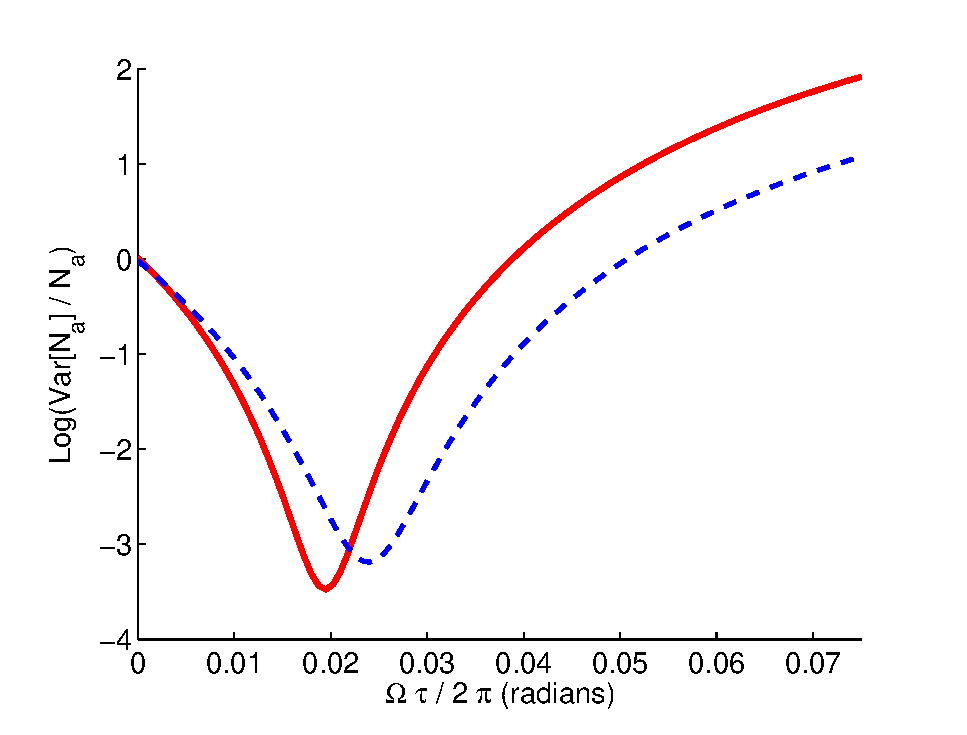
\includegraphics[width=7cm]{figures/realistic_3d_squeezing_params.eps}
\caption{Full 3D simulation of relative number squeezing in state $|a\rangle$ in a system with realistic parameters. Box potential in two dimensions with area 120$\mu$m $\times$ 120$\mu$m, tight harmonic trapping in 3rd dimension with $\omega=1500$Hz. Solid red line, analytic 0D solution; dashed blue line, full 3D multimode simulation. Parameters: Rb$^{85}$ atoms, $n_a = n_b =2 \times 10^5$, $U_{aa}=2.1\times 10^{-50}$ (corresponding to an s-wave scattering length of $-400 a_0$), $U_{bb}=U_{ab}=0$, $\tau_{\mathrm{hold}}=1\times 10^{-3}$s, $\phi=5.3$. Even with all multimode effects present, the number squeezing in the 3D system (13.9dB) approaches that of the ideal 0D case (15.1dB).}
 \label{figRealistic3DParameters}
\end{figure}

\section{Conclusion}
\label{sectionConclusion}
\begin{itemize}
  \item Kerr nonlinearities can give arbitrarily good squeezing in BECs with high number
  \item In a straightforward approach we can't get good squeezing with high number due to MM effects
  \item Mode matching issues can be solved with equal scattering lengths or a pi pulse or a box
  \item Another MM effect scales with dimension and physical size
  \item Can solve that problem with tight trapping and box
\end{itemize}

\ack
Acknowledgements in here; funding sources etc.  Joe's Future Fellowship.  

\clearpage

\appendix
\section{Derivation of two mode squeezing formula}
\label{appendixTwoModeDerivation}
In this Appendix we derive the equations for the number variances. We use the model described in Section \ref{secTwoModeAnalytic}, where we consider a two mode system with $N$ particles, initially prepared as a coherent state with all the population in mode $|a\rangle$ at time $t=0$. A coupling pulse is then applied, so that the system evolves under the Hamiltonian
\begin{equation}
\hat{H_1} = \hbar \omega \hat{a}^{\dagger} \hat{a} +  \hbar \omega \hat{b}^{\dagger} \hat{b} 
          + \Omega (\hat{a}^{\dagger} \hat{b} + \hat{b}^{\dagger} \hat{a} )
\end{equation}
until time $t=t_1$. From time $t_1$ until time $t=t_2$ the coupling is turned off, and the system evolves under the Hamiltonian
\begin{equation}
\hat{H_2} = \frac{\chi_{aa}}{2} \hat{a}^{\dagger} \hat{a}^{\dagger} \hat{a} \hat{a}
          + \chi_{ab} \hat{a}^{\dagger} \hat{a} \hat{b}^{\dagger} \hat{b}
          + \frac{\chi_{bb}}{2} \hat{b}^{\dagger} \hat{b}^{\dagger} \hat{b} \hat{b}.
\end{equation}
Finally, from time $t_2$ until time $t=t_3$, the coupling is once again applied with a phase offset of $\phi$ relative to the first time, and the system evolves via
\begin{equation}
\hat{H_3} = \hbar \omega \hat{a}^{\dagger} \hat{a} +  \hbar \omega \hat{b}^{\dagger} \hat{b}
          + \Omega (e^{i\phi} \hat{a}^{\dagger} \hat{b} + e^{-i\phi} \hat{b}^{\dagger} \hat{a} ).
\end{equation}
It is clear that the linear self-energy terms proportional to $\omega$ result in a constant phase rotation of the fields $\hat{a}$ and $\hat{b}$. As this system is self-contained and global phase is unmeasurable, all phase measurements can only rely on the difference in phase between the two modes. This phase rotation is therefore irrelevent and will be ignored in the following analysis.

We will work in the Heisenberg picture, and derive expressions for $\hat{a}(t_3)$ and $\hat{b}(t_3)$ in terms of $\hat{a}(t_2)$ and $\hat{b}(t_2)$, which in turn can be expressed in terms of $\hat{a}(t_1)$ and $\hat{b}(t_1)$. We will show that the state of the system at time $t_1$ consists of seperate coherent states in modes $|a\rangle$ and $|b\rangle$, enabling us to calculate expectation values at time $t_3$ in terms of the known state at $t_1$.

In order to have more compact expressions we will use the notation
\begin{eqnarray}
\hat{a}(t_j) &=& \hat{a}_j \\
\hat{b}(t_j) &=& \hat{b}_j.
\end{eqnarray}

Beginning with the Hamiltonian $H_1$, during the period $(0, t_1)$ mode $\hat{a}$ will evolve as
\begin{equation}
\hat{a}_1 = e^{ i H_1 t/ \hbar} \, \hat{a}_0 \, e^{-i H_1 t/ \hbar}.
\end{equation}
Utilizing the Hadamard lemma
\begin{equation}
e^X Y e^{-X} = Y + [X,Y] + \frac{1}{2!}[X,[X,Y]] + \frac{1}{3!}[X,[X,[X,Y]]] + \ldots
\label{eqHadamard}
\end{equation}
we obtain 
\begin{eqnarray}
\hat{a}_1 &=& \hat{a}_0 - i \Omega t_1 \hat{b}_0 + \frac{(i \Omega t_1)^2}{2!} \hat{a}_0 - \frac{(i \Omega t_1)^3}{3!} \hat{b}_0 + \frac{(i \Omega t_1)^4}{4!} \hat{a}_2 - \ldots \nonumber \\
          &=& \cos (\Omega t_1) \hat{a}_0 -i \sin (\Omega t_1) \hat{b}_0.
\label{eqa1}
\end{eqnarray}
Similarly, we find
\begin{equation}
\hat{b}_1 = \cos (\Omega t_1) \hat{b}_0 - i \sin (\Omega t_1) \hat{a}_0.
\label{eqb1}
\end{equation}
From the form of (\ref{eqa1}) and (\ref{eqb1}) it is clear that as both modes $\hat{a}$ and $\hat{b}$ began in coherent states, they will remain in coherent states, with only their amplitudes changing. Specifically, at time $t_1$ the system is in a product of coherent states, which we denote $|\alpha, \beta\rangle$ with $\alpha=\sqrt{n_a}$ and $\beta=-i\sqrt{n_b}$.

Next we consider evolution under $H_2$. Taking mode $\hat{a}$ first, we note that as it commutes with the $\hat{b}^{\dagger} \hat{b}^{\dagger} \hat{b} \hat{b}$ term, and since $\hat{a}^{\dagger} \hat{a}^{\dagger} \hat{a} \hat{a}$ commutes with $\hat{a}^{\dagger} \hat{a} \hat{b}^{\dagger} \hat{b}$ we have
\begin{equation}
\hat{a}_2 = e^{i \lambda_{ab} \hat{a}_1^{\dagger} \hat{a}_1 \hat{b}_1^{\dagger} \hat{b}_1 } 
          e^{ i \frac{\lambda_{aa}} {2} \hat{a}_1^{\dagger} \hat{a}_1^{\dagger} \hat{a}_1 \hat{a}_1}\, \hat{a}_1 \,  
          e^{ -i \frac{\lambda_{aa}}{2} \hat{a}_1^{\dagger} \hat {a}_1^{\dagger} \hat{a}_1 \hat{a}_1 }
          e^{-i \lambda_{ab} \hat{a}_1^{\dagger} \hat{a}_1 \hat{b}_1^{\dagger} \hat{b}_1}
\label{eqa2evolution}
\end{equation}
where we have defined $\lambda_{ij} = \chi_{ij} (t_2-t_1)/\hbar$. Utilizing (\ref{eqHadamard}) to move $\hat{a}_1$ through the exponential, with some algebra one can show that
\begin{eqnarray}
e^{ i \frac{\lambda_{aa}} {2} \hat{a}_1^{\dagger} \hat{a}_1^{\dagger} \hat{a}_1 \hat{a}_1} \hat{a}_1 
         e^{ -i \frac{\lambda_{aa}} {2} \hat{a}_1^{\dagger} \hat{a}_1^{\dagger} \hat{a}_1 \hat{a}_1} &=& \left[ \sum_{n=0} (-i \lambda_{aa})^n (\hat{a}_1^{\dagger} \hat{a}_1)^n \right] \hat{a}_1 \nonumber \nonumber \\
   &=& \exp[-i \lambda_{aa} \hat{a}_1^{\dagger} \hat{a}_1] \hat{a}_1.
\end{eqnarray}
To handle the cross-nonlinearity term in (\ref{eqa2evolution}) we use the identity \cite{louisell}
\begin{equation}
e^{x \hat{a}^{\dagger} \hat{a}} f(\hat{a}, \hat{a}^{\dagger}) e^{-x \hat{a}^{\dagger} \hat{a}} = f(\hat{a}e^{-x}, \hat{a}^{\dagger} e^{x})
\label{eqefeidentity}
\end{equation}
to obtain
\begin{eqnarray}
\hat{a}_2 &=& e^{i \lambda_{ab} \hat{a}_1^{\dagger} \hat{a}_1 \hat{b}_1^{\dagger} \hat{b}_1 } 
          e^{-i \lambda_{aa} \hat{a}_1^{\dagger} \hat{a}_1} \, \hat{a}_1 \,
          e^{-i \lambda_{ab} \hat{a}_1^{\dagger} \hat{a}_1 \hat{b}_1^{\dagger} \hat{b}_1} \nonumber \\
%
          &=& e^{-i \lambda_{aa} \hat{a}_1^{\dagger} \hat{a}_1} 
              e^{i \lambda_{ab} \hat{a}_1^{\dagger} \hat{a}_1 \hat{b}_1^{\dagger} \hat{b}_1 } \, \hat{a}_1 \,
          e^{-i \lambda_{ab} \hat{a}_1^{\dagger} \hat{a}_1 \hat{b}_1^{\dagger} \hat{b}_1} \nonumber \\
%
          &=& e^{-i \lambda_{aa} \hat{a}_1^{\dagger} \hat{a}_1} e^{-i \lambda_{ab} \hat{b}_1^{\dagger} \hat{b}_1} \, \hat{a}_1
\label{eqa2}
\end{eqnarray}
Similarly, from permutation symmetry, we have
\begin{equation}
\hat{b}_2 = e^{-i \lambda_{bb} \hat{b}_1^{\dagger} \hat{b}_1} e^{-i \lambda_{ab} \hat{a}_1^{\dagger} \hat{a}_1} \, \hat{b}_1.     
\label{eqb2}
\end{equation}
Finally, to obtain $\hat{a}_3$ and $\hat{b}_3$ we utilize (\ref{eqa1}) and (\ref{eqb1}) with the phase factor attached to the $\hat{b}$ operator to obtain
\begin{eqnarray}
\hat{a}_3 &=& \cos (\Omega (t_3-t_2)) \hat{a}_2 -i e^{i\phi} \sin (\Omega (t_3-t_2)) \hat{b}_2 \label{eqa3} \\
\hat{b}_3 &=& \cos (\Omega (t_3-t_2)) \hat{b}_2 - i e^{-i\phi} \sin (\Omega (t_3-t_2)) \hat{a}_2 \label{eqb3}
\end{eqnarray} 
We are now in a position to evaluate the number variance of the system throughout the period of the final coupling. The number variances of the fields are defined as
\begin{eqnarray}
{\mathrm{Var}}[N_a] &=& \langle \hat{a}^{\dagger}_3 \hat{a}_3 \hat{a}^{\dagger}_3 \hat{a}_3 \rangle - \langle \hat{a}^{\dagger}_3 \hat{a}_3 \rangle ^2 \label{eqNavariance} \\
%
{\mathrm{Var}}[N_b] &=& \langle \hat{b}^{\dagger}_3 \hat{b}_3 \hat{b}^{\dagger}_3 \hat{b}_3 \rangle - \langle \hat{b}^{\dagger}_3 \hat{b}_3 \rangle ^2.
\label{eqNbvariance}
\end{eqnarray}
Making use of (\ref{eqa3}) and using the shorthand notation 
\begin{eqnarray}
s &=& \sin[\Omega (t_3 - t_2)] \\
c &=& \cos[\Omega (t_3 - t_2)]
\end{eqnarray}
we have
\begin{eqnarray}
\hat{a}^{\dagger}_3 \hat{a}_3 &=& \hat{a}^{\dagger}_2 \hat{a}_2 c^2 +  \hat{b}^{\dagger}_2 \hat{b}_2 s^2 + i c s (e^{-i \phi} \hat{b}^{\dagger}_2 \hat{a}_2 - e^{i \phi} \hat{a}^{\dagger}_2 \hat{b}_2) \\
%
%
\hat{a}^{\dagger}_3 \hat{a}_3 \hat{a}^{\dagger}_3 \hat{a}_3 &=& \hat{a}^{\dagger}_2 \hat{a}_2 \hat{a}^{\dagger}_2 \hat{a}_2 c^4 + \hat{b}^{\dagger}_2 \hat{b}_2 \hat{b}^{\dagger}_2 \hat{b}_2 s^4 \nonumber \\
%
&& + c^2 s^2 [ \hat{a}^{\dagger}_2 \hat{a}_2 + \hat{b}^{\dagger}_2 \hat{b}_2 + 4 \hat{a}^{\dagger}_2 \hat{a}_2 \hat{b}^{\dagger}_2 \hat{b}_2 -e^{2 i \phi} \hat{a}^{\dagger}_2 \hat{a}^{\dagger}_2 \hat{b}_2 \hat{b}_2 -e^{-2 i \phi} \hat{b}^{\dagger}_2 \hat{b}^{\dagger}_2 \hat{a}_2 \hat{a}_2 ] \nonumber \\
%
&& + i c^3 s [2 e^{-i \phi} \hat{b}^{\dagger}_2 \hat{a}^{\dagger}_2 \hat{a}_2 \hat{a}_2 - 2 e^{i \phi} \hat{a}^{\dagger}_2 \hat{a}^{\dagger}_2 \hat{a}_2 \hat{b}_2 + e^{-i \phi} \hat{b}^{\dagger}_2 \hat{a}_2 - e^{i \phi} \hat{a}^{\dagger}_2 \hat{b}_2 ] \nonumber \\
%
&& + i c s^3 [2 e^{-i \phi} \hat{b}^{\dagger}_2 \hat{b}^{\dagger}_2 \hat{a}_2 \hat{b}_2 - 2 e^{i \phi} \hat{a}^{\dagger}_2 \hat{b}^{\dagger}_2 \hat{b}_2 \hat{b}_2 + e^{-i \phi} \hat{b}^{\dagger}_2 \hat{a}_2 - e^{i \phi} \hat{a}^{\dagger}_2 \hat{b}_2 ]
\end{eqnarray}
\begin{eqnarray}
\hat{b}^{\dagger}_3 \hat{b}_3 &=& \hat{b}^{\dagger}_2 \hat{b}_2 c^2 +  \hat{a}^{\dagger}_2 \hat{a}_2 s^2 + i c s ( e^{i \phi} \hat{a}^{\dagger}_2 \hat{b}_2 - e^{-i \phi} \hat{b}^{\dagger}_2 \hat{a}_2) \\
%
%
\hat{b}^{\dagger}_3 \hat{b}_3 \hat{b}^{\dagger}_3 \hat{b}_3 &=& \hat{b}^{\dagger}_2 \hat{b}_2 \hat{b}^{\dagger}_2 \hat{b}_2 c^4 + \hat{a}^{\dagger}_2 \hat{a}_2 \hat{a}^{\dagger}_2 \hat{a}_2 s^4 \nonumber \\
%
&& + c^2 s^2 [ \hat{b}^{\dagger}_2 \hat{b}_2 + \hat{a}^{\dagger}_2 \hat{a}_2 + 4 \hat{b}^{\dagger}_2 \hat{b}_2 \hat{a}^{\dagger}_2 \hat{a}_2 - e^{-2 i \phi} \hat{b}^{\dagger}_2 \hat{b}^{\dagger}_2 \hat{a}_2 \hat{a}_2 -e^{2 i \phi} \hat{a}^{\dagger}_2 \hat{a}^{\dagger}_2 \hat{b}_2 \hat{b}_2 ] \nonumber \\
%
&& + i c^3 s [2 e^{i \phi} \hat{a}^{\dagger}_2 \hat{b}^{\dagger}_2 \hat{b}_2 \hat{b}_2 - 2 e^{-i \phi} \hat{b}^{\dagger}_2 \hat{b}^{\dagger}_2 \hat{b}_2 \hat{a}_2 + e^{i \phi} \hat{a}^{\dagger}_2 \hat{b}_2 - e^{-i \phi} \hat{b}^{\dagger}_2 \hat{a}_2 ] \nonumber \\
%
&& + i c s^3 [2 e^{i \phi} \hat{a}^{\dagger}_2 \hat{a}^{\dagger}_2 \hat{b}_2 \hat{a}_2 - 2 e^{-i \phi} \hat{b}^{\dagger}_2 \hat{a}^{\dagger}_2 \hat{a}_2 \hat{a}_2 + e^{i \phi} \hat{a}^{\dagger}_2 \hat{b}_2 - e^{-i \phi} \hat{b}^{\dagger}_2 \hat{a}_2 ] 
\end{eqnarray}
Clearly, to calculate (\ref{eqNavariance}) and (\ref{eqNbvariance}) we will need the expectation values of terms quartic and quadratic in $\hat{a}_2$ and ${\hat{b}_2}$. Specifically, we require $\langle \hat{a}^{\dagger}_2 \hat{a}_2 \rangle$, $\langle \hat{b}^{\dagger}_2 \hat{b}_2 \rangle$,  $\langle \hat{a}^{\dagger}_2 \hat{b}_2 \rangle$, $\langle \hat{a}^{\dagger}_2 \hat{a}_2 \hat{a}^{\dagger}_2 \hat{a}_2 \rangle$, $\langle \hat{b}^{\dagger}_2 \hat{b}_2 \hat{b}^{\dagger}_2 \hat{b}_2 \rangle$ , $\langle \hat{a}^{\dagger}_2 \hat{a}_2 \hat{b}^{\dagger}_2 \hat{b}_2 \rangle$, $\langle \hat{a}^{\dagger}_2 \hat{a}^{\dagger}_2 \hat{b}_2 \hat{b}_2 \rangle$, $\langle \hat{a}^{\dagger}_2 \hat{b}^{\dagger}_2 \hat{a}_2 \hat{a}_2 \rangle$, and $\langle \hat{a}^{\dagger}_2 \hat{b}^{\dagger}_2 \hat{b}_2 \hat{b}_2 \rangle$, as well as their Hermitian conjugates.

As $\hat{a}^{\dagger}_1 \hat{a}_1$ and $\hat{b}^{\dagger}_1 \hat{b}_1$ commute with the Hamiltonian $H_2$, they are constants of motion so we have
\begin{equation}
\langle \hat{a}^{\dagger}_2 \hat{a}_2 \rangle = \langle \hat{a}^{\dagger}_1 \hat{a}_1 \rangle = \langle \alpha, \beta | \hat{a}^{\dagger}_1 \hat{a}_1 |\alpha, \beta \rangle = |\alpha|^2 = n_a
\end{equation}
%
\begin{equation}
\langle \hat{b}^{\dagger}_2 \hat{b}_2 \rangle = \langle \hat{b}^{\dagger}_1 \hat{b}_1 \rangle = \langle \alpha, \beta | \hat{b}^{\dagger}_1 \hat{b}_1 |\alpha, \beta \rangle = |\beta|^2 = n_b
\end{equation}
%
\begin{equation}
\langle \hat{a}^{\dagger}_2 \hat{a}_2 \hat{b}^{\dagger}_2 \hat{b}_2 \rangle = \langle \hat{a}^{\dagger}_1 \hat{a}_1 \hat{b}^{\dagger}_1 \hat{b}_1 \rangle = \langle \alpha, \beta | \hat{a}^{\dagger}_1 \hat{a}_1 \hat{b}^{\dagger}_1 \hat{b}_1 |\alpha, \beta \rangle = |\alpha|^2 |\beta|^2 = n_a n_b
\end{equation}
Furthermore, $\hat{a}^{\dagger}_2 \hat{a}_2 \hat{a}^{\dagger}_2 \hat{a}_2$ and $\hat{b}^{\dagger}_2 \hat{b}_2 \hat{b}^{\dagger}_2 \hat{b}_2$ also commute with $H_2$, giving
\begin{equation}
\langle \hat{a}^{\dagger}_2 \hat{a}_2 \hat{a}^{\dagger}_2 \hat{a}_2 \rangle = \langle \hat{a}^{\dagger}_1 \hat{a}_1 \hat{a}^{\dagger}_1 \hat{a}_1 \rangle = \langle \alpha, \beta | \hat{a}^{\dagger}_1 \hat{a}^{\dagger}_1 \hat{a}_1 \hat{a}_1 + \hat{a}^{\dagger}_1 \hat{a}_1 |\alpha, \beta \rangle = n_a^2 + n_a
\end{equation}
%
\begin{equation}
\langle \hat{b}^{\dagger}_2 \hat{b}_2 \hat{b}^{\dagger}_2 \hat{b}_2 \rangle = \langle \hat{b}^{\dagger}_1 \hat{b}_1 \hat{b}^{\dagger}_1 \hat{b}_1 \rangle = \langle \alpha, \beta | \hat{b}^{\dagger}_1 \hat{b}^{\dagger}_1 \hat{b}_1 \hat{b}_1 + \hat{b}^{\dagger}_1 \hat{b}_1 |\alpha, \beta \rangle = n_b^2 + n_b
\end{equation}
The remaining terms are not constants of motion, so we proceed by making use of (\ref{eqa2}) and (\ref{eqb2}). For $\langle \hat{a}^{\dagger}_2 \hat{b}_2 \rangle$ we have
\begin{equation}
\hat{a}^{\dagger}_2 \hat{b}_2 = \hat{a}^{\dagger}_1 e^{-i (\lambda_{bb} - \lambda_{ab}) \hat{b}^{\dagger}_1 \hat{b}_1} e^{i (\lambda_{aa} - \lambda_{ab}) \hat{a}^{\dagger}_1 \hat{a}_1} \hat{b}_1. 
\end{equation}
To calculate the expectation value of this expression, the creation and annihilation operators must be normally ordered. Making use of the identity \cite{louisell}
\begin{equation}
e^{x \hat{a}^{\dagger} \hat{a}} = \sum_{n=0}^{\infty} \frac{(e^x - 1)^n} {n!} (\hat{a}^{\dagger})^n (\hat{a})^n
\end{equation}
allows us to compute expectation values of coherent states of the form
\begin{eqnarray}
\langle \alpha | e^{x \hat{a}^{\dagger} \hat{a}} |\alpha \rangle &=& \sum_{n=0}^{\infty} \frac{(e^x - 1)^n} {n!} |\alpha|^{2n} \nonumber \\
%
&=& \exp[|\alpha|^2(e^x -1)]. \label{eqExpectationValueOfExponential}
\end{eqnarray}
This gives
\begin{eqnarray}
\langle \hat{a}^{\dagger}_2 \hat{b}_2 \rangle &=& \langle \alpha, \beta | \hat{a}^{\dagger}_1 e^{-i (\lambda_{bb} - \lambda_{ab}) \hat{b}^{\dagger}_1 \hat{b}_1} e^{i (\lambda_{aa} - \lambda_{ab}) \hat{a}^{\dagger}_1 \hat{a}_1} \hat{b}_1 | \alpha, \beta \rangle \nonumber \\
%
&=& \alpha^* \beta \exp[|\alpha|^2(e^{i (\lambda_{aa} - \lambda_{ab})} -1)] \exp[|\beta|^2 (e^{-i (\lambda_{bb} - \lambda_{ab})} -1)].
\end{eqnarray}

Next we tackle $\langle \hat{a}^{\dagger}_2 \hat{a}^{\dagger}_2 \hat{b}_2 \hat{b}_2 \rangle$. Using (\ref{eqa2}) and (\ref{eqb2}) and the fact that $\hat{a}$ and $\hat{b}$ commute, we have
\begin{eqnarray}
\hat{a}^{\dagger}_2 \hat{a}^{\dagger}_2 \hat{b}_2 \hat{b}_2 &=& \hat{a}^{\dagger}_1 
  e^{i (\lambda_{aa}-\lambda_{ab}) \hat{a}^{\dagger}_1 \hat{a}_1}
  \hat{b}_1 \hat{a}^{\dagger_1}
  e^{i (\lambda_{ab}-\lambda_{bb}) \hat{b}^{\dagger}_1 \hat{b}_1}
  e^{i (\lambda_{aa}-\lambda_{ab}) \hat{a}^{\dagger}_1 \hat{a}_1}
  \hat{b}_1 \\
%
&=& \hat{a}^{\dagger}_1 \hat{a}^{\dagger}_1 
    e^{2i (\lambda_{aa}-\lambda_{ab}) \hat{a}^{\dagger}_1 \hat{a}_1}
    e^{2i (\lambda_{ab}-\lambda_{bb}) \hat{b}^{\dagger}_1 \hat{b}_1}
    \hat{b}_1 \hat{b}_1 e^{i(\lambda_{aa}-\lambda_{bb})}
\end{eqnarray}
where we have made multiple uses of the identity 
\begin{equation}
\hat{a} e^{i x \hat{a}^{\dagger} \hat{a}} = e^{i x \hat{a}^{\dagger} \hat{a}} \hat{a} e^{ix}
\end{equation}
which follows from (\ref{eqefeidentity}). Finally, applying (\ref{eqExpectationValueOfExponential}) we obtain
\begin{equation}
\langle \hat{a}^{\dagger}_2 \hat{a}^{\dagger}_2 \hat{b}_2 \hat{b}_2 \rangle = \alpha^{*2} \beta^2 e^{i(\lambda_{aa}-\lambda_{bb})} \exp[|\alpha|^2(e^{2i (\lambda_{aa} - \lambda_{bb})} -1)] \exp[|\beta|^2(e^{-2i (\lambda_{bb} - \lambda_{bb})} -1)].
\end{equation}
Using the same techniques one can show that
\begin{eqnarray}
\langle \hat{a}^{\dagger}_2 \hat{b}^{\dagger}_2 \hat{a}_2 \hat{a}_2 \rangle &=& |\alpha|^2 \alpha \beta^* e^{-i(\lambda_{aa}-\lambda_{ab})} \exp[|\alpha|^2(e^{-i (\lambda_{aa} - \lambda_{ab})} -1)] \exp[|\beta|^2(e^{i (\lambda_{bb} - \lambda_{ab})} -1)] \\
%
\langle \hat{a}^{\dagger}_2 \hat{b}^{\dagger}_2 \hat{b}_2 \hat{b}_2 \rangle &=& |\beta|^2 \alpha^{*} \beta e^{-i(\lambda_{bb}-\lambda_{ab})} \exp[|\alpha|^2(e^{i (\lambda_{aa} - \lambda_{ab})} -1)] \exp[|\beta|^2(e^{-i (\lambda_{bb} - \lambda_{ab})} -1)].
\end{eqnarray}
Employing the definitions (\ref{eqsDef})--(\ref{eqDDef}) we obtain
\begin{eqnarray}
\langle \hat{a}^{\dagger}(t_3) \hat{a}(t_3) \rangle &=& n_a c^2 + n_b s^2 + i c s (A B^* - A^* B) \\
%
\langle \hat{b}^{\dagger}(t_3) \hat{b}(t_3) \rangle &=& n_a s^2 + n_b c^2 - i c s (A B^* - A^* B) \\
%
\langle \hat{a}^{\dagger}(t_3) \hat{a}(t_3) \hat{a}^{\dagger}(t_3)  \hat{a}(t_3) \rangle &=& (n_a^2 + n_a) c^4 + (n_b^2 + n_b) s^4 \nonumber \\
&& + c^2 s^2 [n_a +n_b +4 n_a n_b - e^{i(\lambda_{aa}-\lambda_{bb})} B_2 A_2^* - e^{-i(\lambda_{aa}-\lambda_{bb})} B_2^* A_2] \nonumber \\
&& + i c^3 s [2 n_a e^{-i(\lambda_{aa}-\lambda_{ab})}] A B^* - 2 n_a e^{i(\lambda_{aa}-\lambda_{ab})} A^* B + A B^* - A^* B] \nonumber \\
&& + i c s^3 [2 n_b e^{i(\lambda_{bb}-\lambda_{ab})}] A B^* - 2 n_b e^{-i(\lambda_{bb}-\lambda_{ab})} A^* B + A B^* - A^* B] \\
%
\langle \hat{b}^{\dagger}(t_3)  \hat{b}(t_3) \hat{b}^{\dagger}(t_3)  \hat{b}(t_3) \rangle &=& (n_b^2 + n_b) c^4 + (n_a^2 + n_a) s^4 \nonumber \\
&& + c^2 s^2 [n_a +n_b +4 n_a n_b - e^{-i(\lambda_{aa}-\lambda_{bb})} B_2^* A_2 - e^{i(\lambda_{aa}-\lambda_{bb})} B_2 A_2^*] \nonumber \\
&& + i c^3 s [2 n_b e^{-i(\lambda_{bb}-\lambda_{ab})}] A^* B - 2 n_b e^{i(\lambda_{bb}-\lambda_{ab})} A B^* - A^* B + A B^*] \nonumber \\
&& + i c s^3 [2 n_a e^{i(\lambda_{aa}-\lambda_{ab})}] A^* B - 2 n_a e^{-i(\lambda_{aa}-\lambda_{ab})} A B^* - A^* B + A B^*]. 
\end{eqnarray}
When substituted into (\ref{eqNavariance}) and (\ref{eqNbvariance}) these expecation values give the absolute number variances stated in Section \ref{secTwoModeAnalytic}. To calculate the number difference variance, we note
\begin{equation}
{\mathrm{Var}}[N_a-N_b] = {\mathrm{Var}}[N_a] + {\mathrm{Var}}[N_b] - 2\langle \hat{a}^{\dagger}_3 \hat{a}_3 \hat{b}^{\dagger}_3 \hat{b}_3\rangle + 2\langle \hat{a}^{\dagger}_3  \hat{a}_3 \rangle \langle \hat{b}^{\dagger}_3 \hat{b}_3\rangle \label{eqNumDiffVarianceAppendix}.
\end{equation}
We write (\ref{eqNumDiffVarianceAppendix}) in terms of $\hat{a}_2$ and $\hat{b}_2$ by using using (\ref{eqa3}) and (\ref{eqb3}), and then use the expectation values calculated earlier in this Appendix. After some algebra we obtain the expression (\ref{eqNumDiffVariance}) given in Section \ref{secTwoModeAnalytic}.

\section{Derivation of Bogoliubov squeezing formula}
\label{appendixBogDerivation}

Here we put some details of the Bog analysis.

\begin{align}
  S &= \frac{\Var(n_0) + \sum_k \frac{1}{2} n_k (3 + \cos 2\theta + 4 n_k)}{n_0 + \sum_k n_k} \\
  n_k &= \left[\lambda \cos\theta \sinc(\omega_k \tau)\right]^2 \\
  \hat{a}(t_3) &= \left[\hat{a}(0) - i \chi \alpha \tau_h\left(\alpha^* \hat{a}(0) + \alpha \hat{a}^\dagger(0) - 2\abs{\alpha}^2\right) \right]\cos(\theta) - i\hat{b}(0) \sin\theta e^{i\phi} \\
  n_0 &= \left(\alpha ^2+\alpha ^4 \lambda ^2\right) \cos^2\theta + \left(\beta^2 \sin\theta  + 2\alpha\beta\cos\theta\sin\phi\right)\sin\theta\\
  \begin{split}
  \Var(n_0) &= \frac{1}{2} \left(\alpha ^2+\beta ^2\right)+\frac{1}{8}\alpha ^4 \left(7+ 2\beta ^2\right) \lambda ^2+ \frac{3}{4} \alpha ^8 \lambda ^4 \\
  &\phantom{\mathrel{=}}+\frac{1}{2}\left( \alpha ^2-\beta ^2+2 \alpha ^4 \lambda ^2+2 \alpha ^8 \lambda ^4\right) \text{Cos}[2 \theta ] \\
  &\phantom{\mathrel{=}}+\frac{1}{8}\left(\alpha ^4 \lambda ^2 \left(1-2 \beta ^2+2 \alpha ^4 \lambda ^2\right) \text{Cos}[4 \theta ] \right) \\
  &\phantom{\mathrel{=}}+\frac{1}{8}\left(4 \alpha  \beta  \left(8 \alpha ^2 \lambda  \text{Cos}[\theta ]^3 \text{Cos}[\phi ] \text{Sin}[\theta ]+\text{Sin}[2 \theta ] \left(2 \text{Sin}[\phi ]+\alpha  \beta  \lambda  \text{Sin}[2 \theta ] \left(\alpha ^2 \lambda  \text{Cos}[2 \phi ]+\text{Sin}[2 \phi ]\right)\right)\right)\right)
  \end{split}
\end{align}


\section*{References}
\begin{thebibliography}{10}
\bibitem{Hadzibabic2004} Hadzibabic Z, Stock S, Battelier B, Bretin V and Dalibard J 2004 Interference of an array of independent Bose-Einstein Condensates {\it Phys. Rev. Lett.} {\bf 93} 180403
\bibitem{johnssonET2007} Johnsson M T and Haine S A 2007 Generating squeezing in an atom laser through self-interaction {\it Phys. Rev. Lett.} {\bf 99} 010401

\bibitem{dallET2009} Dall R G, Byron L J, Truscott A G, Dennis G R, Johnsson M T and Hope J J 2009 Paired-atom laser beams created via four-wave mixing {\it Phys. Rev. A} {\bf 79} 011601(R)

\bibitem{dennisET2010} Dennis G R and Johnsson M T 2010 Generation of directional coherent matter beams through dynamical instabilities in Bose-Einstein condensates {\it Phys. Rev. A} {\bf 82} 033615


\bibitem{dennis2013} Dennis G R, Hope J J and Johnsson M T 2013 XMDS2: Fast, scalable simulation of coupled stochastic partial
differential equations {\it Comput. Phys. Commun.} {\bf 184} 201--208
\bibitem{louisell} Louisell Quantum Statistical Properties of Radiation

\bibitem{gross2010} Gross C, Zibold T, Est{\`{e}}ve J and Oberthaler M K 2010 Nonlinear atom interferometer surpasses classical
precision limit {\it Nature} {\bf 464} 1165--1169

\bibitem{PethickSmith} C.J.~Pethick and H.~Smith, \emph{Bose-Einstein Condensation in Dilute Gases} (Cambridge University Press, Cambridge, 2002).

\end{thebibliography}

\end{document}

